\documentclass[10pt,a4paper]{article}

%double si on veut une version prof et une version élève. simple si on veut une seule version.
\newcommand{\buildmode}{double}

\InputIfFileExists{version.tex}{}{}
% Version (définie par le script)
\providecommand{\version}{eleve}

\usepackage{feuilleactivite}

%%%à modifier à chaque fois

\renewcommand{\niveau}{2nde}
\renewcommand{\chapitre}{Fonctions, généralités}
\renewcommand{\numchap}{0.1} 
\renewcommand{\theme}{Fonctions}

\begin{document}


%\legendeicones

\vspace{-0.3cm}

\begin{objectifs}
\begin{itemize}
    \item Lire et comprendre un graphique comme la représentation d'une fonction.
    \item Se réapproprier le vocabulaire des fonction.
    \item Lire et compléter un tableau de valeurs.
    \item Tracer une fonction à partir d'un tableau de valeurs.
\end{itemize}
\end{objectifs}

\prof{En fonction du temps qu'il reste, pour les bons élèves. On peut ajouter des exercices au tableau, par exemple\begin{itemize}
    \item Tracer une fonction, calculer \(f(2)\), donner l'image d'un nombre, ses antécédents, résoudre une équation et coordonnée de points.
    \item Tableau de valeurs avec des variables didatiques plus difficiles (relatifs et \(\dfrac{1}{2}\))
\end{itemize}}

\section{Courbe de température}

Le graphique ci-dessous représente l'évolution de la température en °C à Saint-Denis le 15 août 2026. 

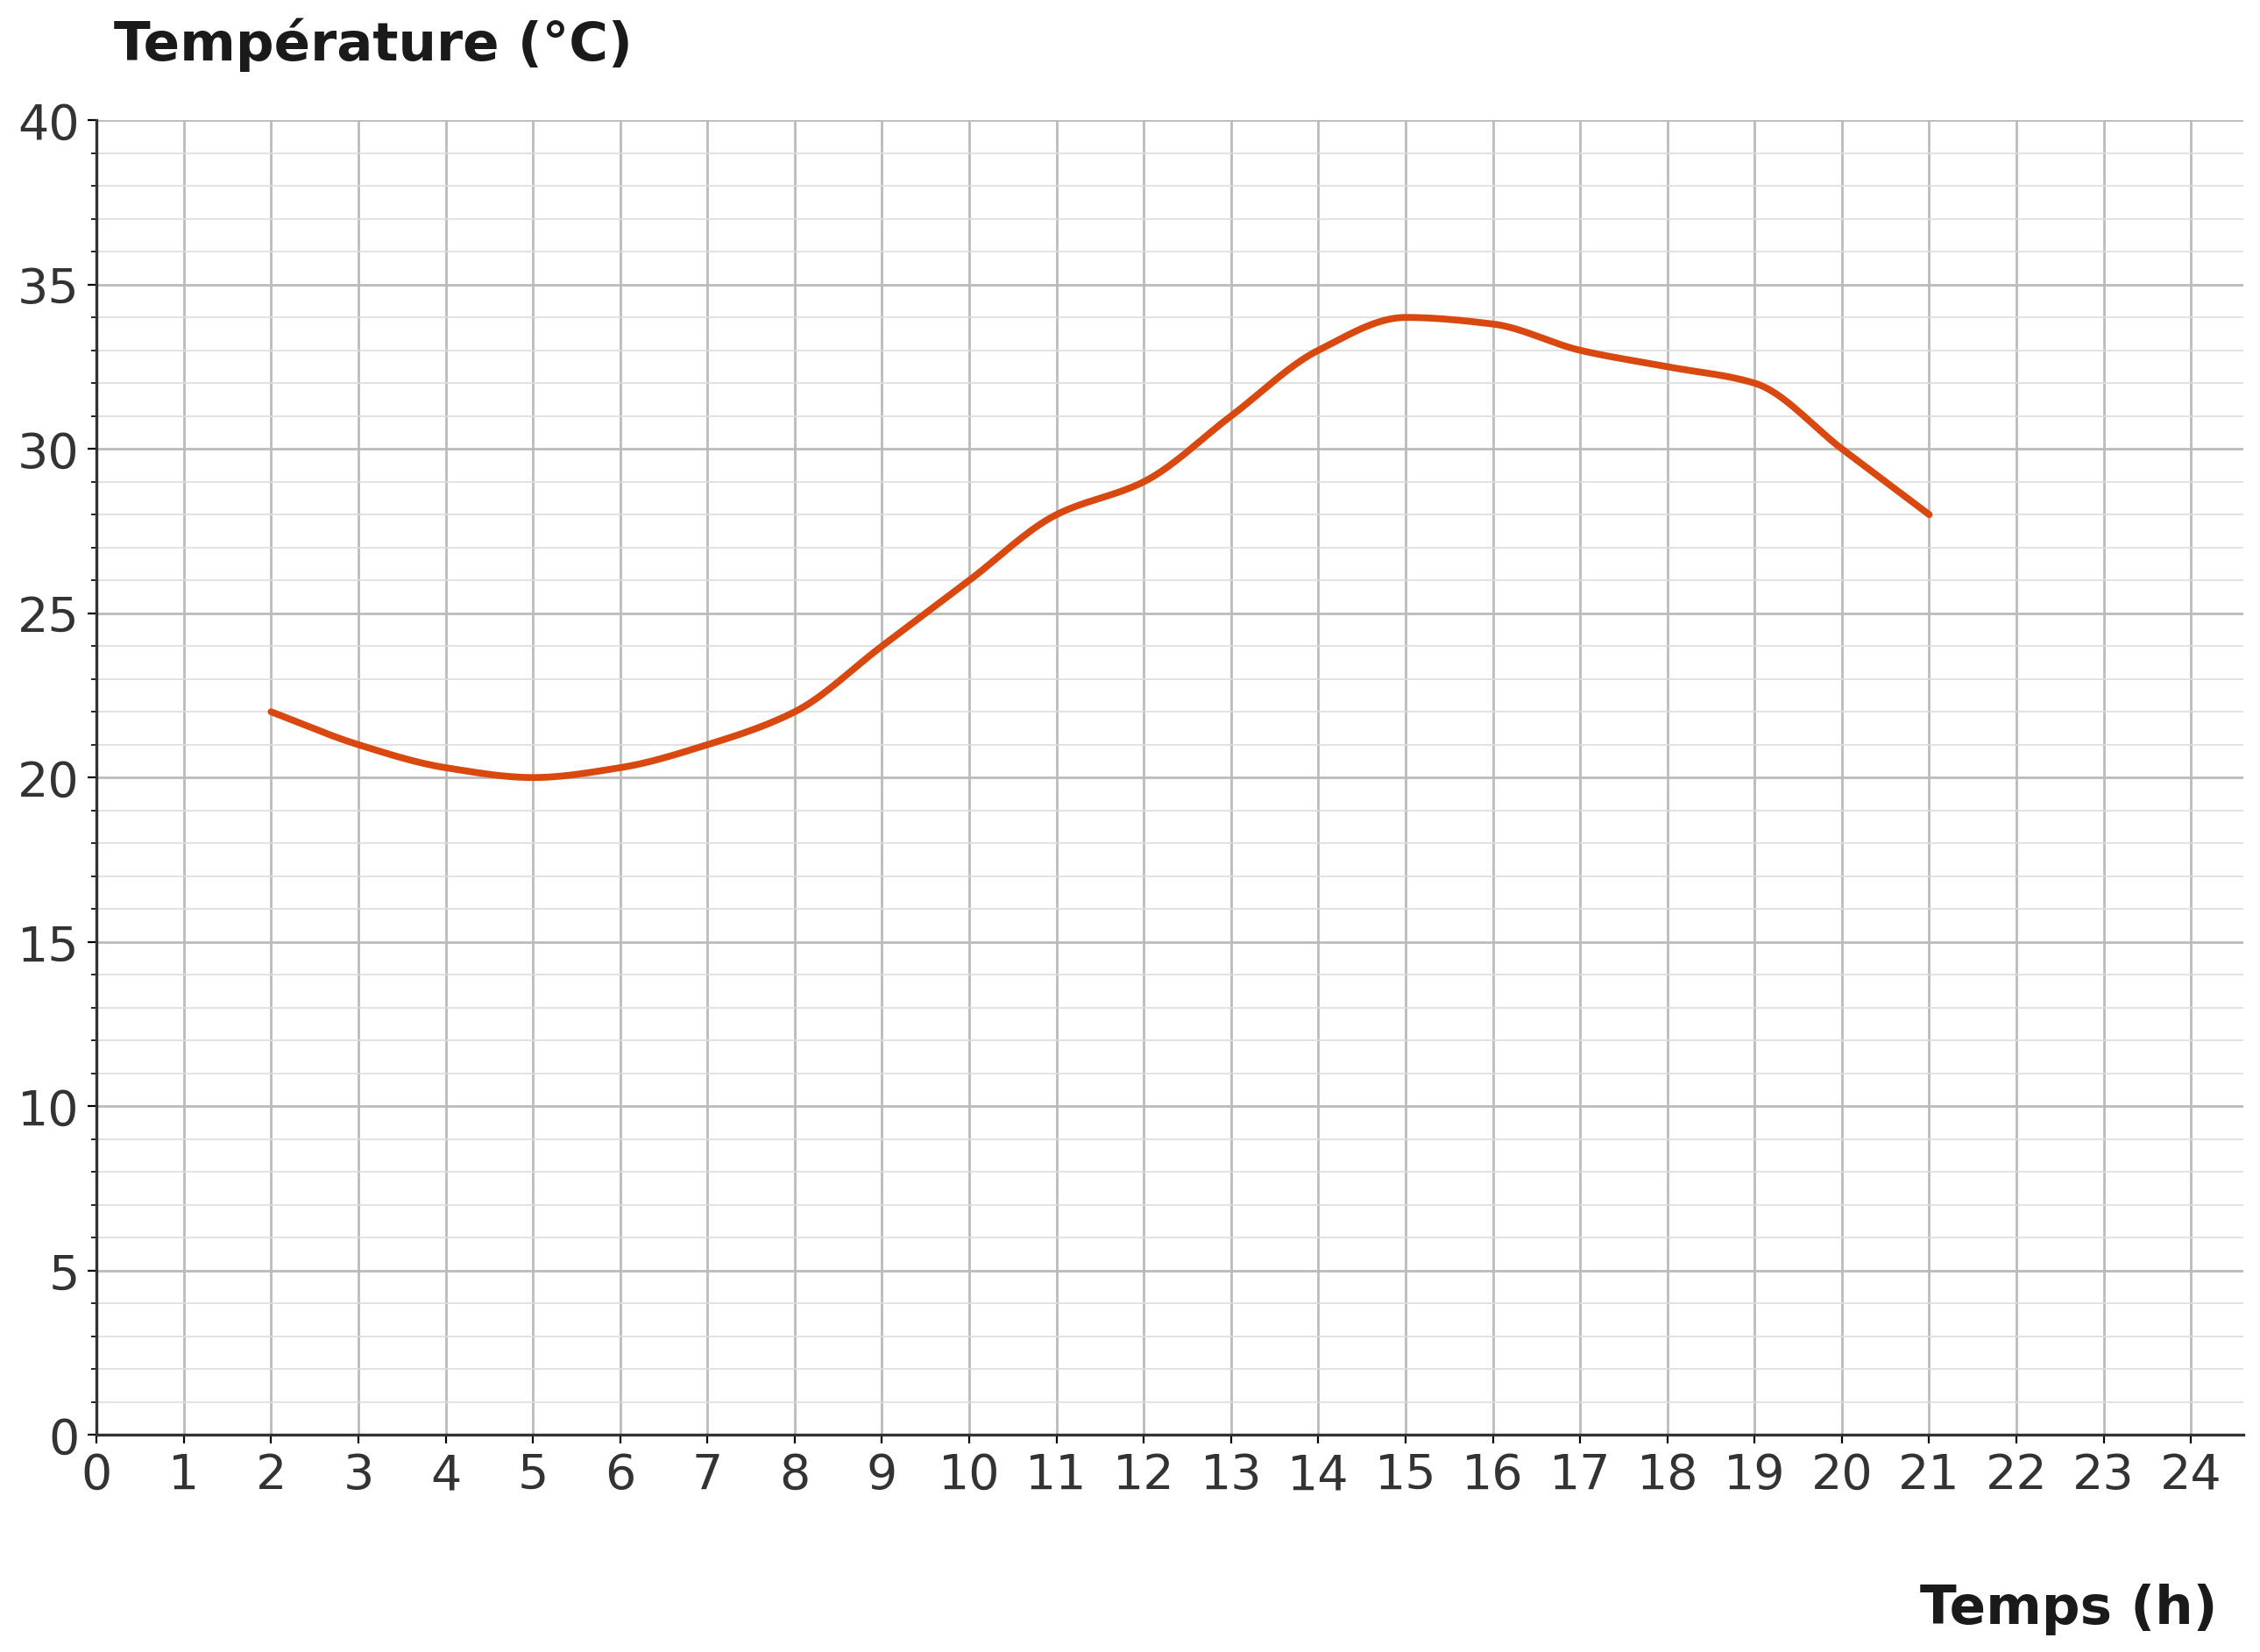
\includegraphics[width=0.8\textwidth]{saint_denis_93_temp_full_axis.png}

\begin{enumerate}

    \item Utilisez le graphique pour répondre aux questions suivantes :
    \renewcommand{\arraystretch}{2} %donne la distance entre les lignes%
    %\setlength{\tabcolsep}{1cm} %donne la distance entre les colonnes%
    \begin{center}
    \begin{tabular}{|p{5cm}|p{10cm}|}
    \hline
    Questions & Réponses \\
    \hline
    \hline
    Sur quels horaires les températures ont-elles été relevées ? & \\
    \hline
    Quelle était la température à 7h du matin ? &    \\
    \hline
    A quelles heures la température était-elle de 30°C ? &  \\
    \hline
    Sur quelles plages horaires la température a-t-elle diminué ? & \\ 
    \hline
    Entre 9h et midi, la température a-t-elle augmenté ou diminué ?& \\ 
    \hline
    Donner les températures extrêmes. A quelles heures ont-elles pu être observées ?  & \\
    \hline
    \end{tabular}
    \end{center}


    \item Listez tous les mots de vocabulaire dont vous vous souvenez de l'année de seconde sur les fonctions (par exemple : antécédent). 
    \prof{
        Mise en commun au tableau. On attend au moins : image, antécédent, ensemble de définition, croissant, maximum.

        Définir la fonction température avec les élèves et l'appeler \(f\). Réfléchir aux variables didactiques, \(t\) ou \(f\).
    }

    \medskip

    \textit{\underline{Commentaire :} On considérera maintenant que la température est une fonction du temps, que l'on notera \(f\)}

    \medskip


    \item Le tableau ci-dessous est le même que celui de la question 1, mais reformulé avec le vocabulaire des fonctions. Complétez-le.
    


        \begin{center}
    \begin{tabular}{|p{5cm}|p{10cm}|}
    \hline
    Questions & Réponses \\
    \hline
    \hline
    Quel est l'ensemble de définition de la fonction ? & L'ensemble de définition de la fonction est l'intervalle \([2\ ;\; 21]\) \\
    \hline
     Quelle est l'image de 7 par la fonction \(f\) ? &  \vspace{0.5cm}   \\
    \hline
    \vspace{0.5cm} &  \\
    \hline
    Sur quelles intervalles la température est-elle décroissante ? & \vspace{0.5cm} \\ 
    \hline
    \vspace{0.5cm}  & La température est croissante sur l'intervalle \([9\ ; \ 12]\)  \\ 
    \hline
     \vspace{0.5cm} &  \\
    \hline
    \end{tabular}
    \end{center}
    
\end{enumerate}

\section{Tableau de valeur}
On considère la fonction \(f\) définie sur l'intervalle \([0\ ;\ 5]\) par \(f(x)=x^2-2x+3\). 


\begin{multicols}{2}
    \begin{minipage}{0.45\textwidth}
    \begin{enumerate}
    \item Complétez le tableau de valeurs suivant.
    
    \begin{center}
        \renewcommand{\arraystretch}{1.5} %donne la distance entre les lignes%
        \setlength{\tabcolsep}{0.3cm} %donne la distance entre les colonnes%
        \begin{tabular}{|c|c|c|c|c|c|c|}
        \hline
        \(x\) & 0 & 1 & 2 & 3 & 4 & 5 \\
        \hline
        \(f(x)\) &  &  &  &  &  &  \\
        \hline
        \end{tabular}
    \end{center}

    \vfill\null
    
    \item À l'aide du tableau, tracer la courbe représentative de la fonction.
    \end{enumerate}

    \vspace{1cm}

    \section{Programme de calcul}

    Voici un programme de calcul : 

    \begin{verbatim}
        Choisissez un nombre
        Multipliez le par 5
        Ajoutez 3 au résultat.
    \end{verbatim}
    \begin{enumerate}
        \item Comment peut-on écrire une fonction associée à ce programme ?
        \item Quelle est l'image de 1,5 ?
        \item Quelle est l'image de -1 ?
        \item Peut-on trouver un nombre qui aura pour image zéro ?
    \end{enumerate}
    \end{minipage}


     \vfill\null
    
    \hspace{-1cm}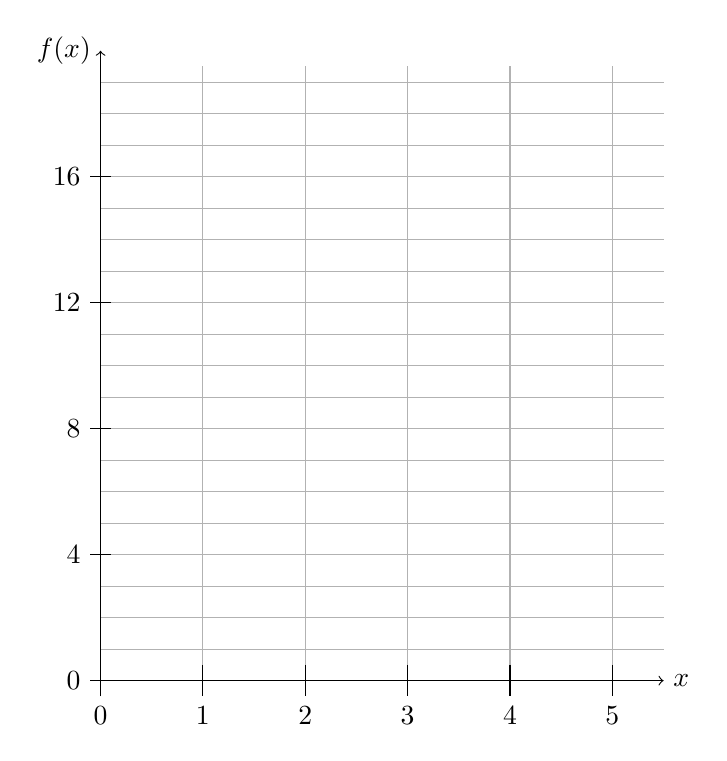
\begin{tikzpicture}[yscale=0.4, xscale=1.3]
        \draw[step=1.0,black!30!white,thin] (0,0) grid (5.5,19.5);
        \draw[->] (-0.1,0) -- (5.5,0) node[right] {\(x\)};
        \draw[->] (0,-0.5) -- (0,20) node[left] {\(f(x)\)};
        \foreach \x in {0,1,2,3,4,5} \draw (\x,0.5) -- (\x,-0.5) node[below] {\(\x\)};
        \foreach \y in {0,4,...,16} \draw (0.1,\y) -- (-0.1,\y) node[left] {\(\y\)};
    \end{tikzpicture}


\end{multicols}


\end{document}
